\documentclass[11pt,a4paper]{article}

% no build date or random ID in the PDF, so a rebuild is byte for byte the same
\pdfinfoomitdate=1
\pdftrailerid{}
\pdfsuppressptexinfo=-1

\usepackage[margin=2cm]{geometry}
\usepackage[T1]{fontenc}
\usepackage{lmodern}
\usepackage{microtype}
\usepackage{amsmath}
\usepackage{array}
\usepackage{booktabs}
\usepackage{multirow}
\usepackage{graphicx}
\usepackage{float}
\usepackage{caption}
\usepackage[hidelinks]{hyperref}

\captionsetup{font=small,labelfont=bf}
\setlength{\parskip}{4pt}
\setlength{\parindent}{0pt}

% Every number comes from results/numbers.tex, which `python -m tools.run_all` writes from what
% the two scripts compute and print; a mistyped key prints a bold ?? and logs MISSING NUMBER.
\makeatletter
\newcommand{\resdef}[2]{\@namedef{res@#1}{#2}}
\newcommand{\res}[1]{\@ifundefined{res@#1}{\typeout{MISSING NUMBER #1}\textbf{??}}%
  {\@nameuse{res@#1}}}
\makeatother
% Written by python -m tools.run_all from results/results.json; do not edit.
\resdef{gc-lrelu}{3.5 \times 10^{-10}}
\resdef{gc-lrelu-rows}{0--4}
\resdef{gc-tanh}{8.0 \times 10^{-11}}
\resdef{gc-tanh-rows}{0--4}
\resdef{t2-lrelu-1-loss}{0.2887}
\resdef{t2-lrelu-1-after}{0.2887}
\resdef{t2-lrelu-1-train}{87.25}
\resdef{t2-lrelu-1-test}{88.00}
\resdef{t2-lrelu-2-loss}{0.2787}
\resdef{t2-lrelu-2-after}{0.2787}
\resdef{t2-lrelu-2-train}{88.25}
\resdef{t2-lrelu-2-test}{88.00}
\resdef{t2-lrelu-8-loss}{0.2607}
\resdef{t2-lrelu-8-after}{0.2606}
\resdef{t2-lrelu-8-train}{87.50}
\resdef{t2-lrelu-8-test}{89.00}
\resdef{t2-lrelu-32-loss}{0.0891}
\resdef{t2-lrelu-32-after}{0.0891}
\resdef{t2-lrelu-32-train}{98.25}
\resdef{t2-lrelu-32-test}{94.00}
\resdef{t2-tanh-1-loss}{0.2925}
\resdef{t2-tanh-1-after}{0.2925}
\resdef{t2-tanh-1-train}{87.25}
\resdef{t2-tanh-1-test}{88.00}
\resdef{t2-tanh-2-loss}{0.2901}
\resdef{t2-tanh-2-after}{0.2901}
\resdef{t2-tanh-2-train}{87.25}
\resdef{t2-tanh-2-test}{88.00}
\resdef{t2-tanh-8-loss}{0.1456}
\resdef{t2-tanh-8-after}{0.1456}
\resdef{t2-tanh-8-train}{95.50}
\resdef{t2-tanh-8-test}{94.00}
\resdef{t2-tanh-32-loss}{0.0986}
\resdef{t2-tanh-32-after}{0.0986}
\resdef{t2-tanh-32-train}{97.25}
\resdef{t2-tanh-32-test}{95.00}
\resdef{linear-train}{87.25}
\resdef{linear-test}{88.00}
\resdef{t3-1-logistic-train}{85.83}
\resdef{t3-1-logistic-test}{83.33}
\resdef{t3-1-logistic-loss}{0.3892}
\resdef{t3-1-logistic-norm}{19.4912}
\resdef{t3-1-relu-train}{99.17}
\resdef{t3-1-relu-test}{97.50}
\resdef{t3-1-relu-loss}{0.0331}
\resdef{t3-1-relu-norm}{16.4026}
\resdef{t3-2-logistic-train}{99.17}
\resdef{t3-2-logistic-test}{97.50}
\resdef{t3-2-logistic-loss}{0.0400}
\resdef{t3-2-logistic-norm}{16.7455}
\resdef{t3-2-relu-train}{98.96}
\resdef{t3-2-relu-test}{99.17}
\resdef{t3-2-relu-loss}{0.0163}
\resdef{t3-2-relu-norm}{7.2583}
\resdef{t3-3-logistic-train}{74.17}
\resdef{t3-3-logistic-test}{75.83}
\resdef{t3-3-logistic-loss}{0.5045}
\resdef{t3-3-logistic-norm}{9.0309}
\resdef{t3-3-relu-train}{98.96}
\resdef{t3-3-relu-test}{97.50}
\resdef{t3-3-relu-loss}{0.0165}
\resdef{t3-3-relu-norm}{4.3625}
\resdef{t3-6-logistic-train}{64.17}
\resdef{t3-6-logistic-test}{66.67}
\resdef{t3-6-logistic-loss}{0.6531}
\resdef{t3-6-logistic-norm}{13.4539}
\resdef{t3-6-relu-train}{98.96}
\resdef{t3-6-relu-test}{98.33}
\resdef{t3-6-relu-loss}{0.0184}
\resdef{t3-6-relu-norm}{2.4838}
\resdef{t4-2-logistic-train}{62.92}
\resdef{t4-2-logistic-test}{64.17}
\resdef{t4-2-logistic-gap}{\textminus{}1.25}
\resdef{t4-2-P}{15}
\resdef{t4-2-relu-train}{66.88}
\resdef{t4-2-relu-test}{60.83}
\resdef{t4-2-relu-gap}{+6.05}
\resdef{t4-4-logistic-train}{61.25}
\resdef{t4-4-logistic-test}{58.33}
\resdef{t4-4-logistic-gap}{+2.92}
\resdef{t4-4-P}{37}
\resdef{t4-4-relu-train}{76.04}
\resdef{t4-4-relu-test}{79.17}
\resdef{t4-4-relu-gap}{\textminus{}3.13}
\resdef{t4-16-logistic-train}{76.67}
\resdef{t4-16-logistic-test}{75.00}
\resdef{t4-16-logistic-gap}{+1.67}
\resdef{t4-16-P}{337}
\resdef{t4-16-relu-train}{99.17}
\resdef{t4-16-relu-test}{99.17}
\resdef{t4-16-relu-gap}{+0.00}
\resdef{t4-64-logistic-train}{98.96}
\resdef{t4-64-logistic-test}{98.33}
\resdef{t4-64-logistic-gap}{+0.63}
\resdef{t4-64-P}{4417}
\resdef{t4-64-relu-train}{99.17}
\resdef{t4-64-relu-test}{98.33}
\resdef{t4-64-relu-gap}{+0.84}
\resdef{t3-6-logistic-minloss}{0.6529}
\resdef{t3-6-relu-minloss}{0.0144}
\resdef{evo-logistic-1}{50.42}
\resdef{evo-logistic-25}{62.29}
\resdef{evo-logistic-100}{61.04}
\resdef{evo-logistic-300}{53.12}
\resdef{evo-logistic-1000}{96.25}
\resdef{evo-relu-1}{50.83}
\resdef{evo-relu-25}{71.46}
\resdef{evo-relu-100}{98.54}
\resdef{evo-relu-300}{98.96}
\resdef{evo-relu-1000}{98.96}
\resdef{python}{3.12.10}
\resdef{numpy}{2.5.5}
\resdef{sklearn}{1.9.1}
\resdef{matplotlib}{3.11.2}


% one row of Table 2, 3 and 4
\newcommand{\rowtwo}[1]{\res{t2-#1-loss} & \res{t2-#1-train} & \res{t2-#1-test}}
\newcommand{\rowthree}[1]{\res{t3-#1-train} & \res{t3-#1-test} & \res{t3-#1-loss} & \res{t3-#1-norm}}
\newcommand{\rowfour}[1]{\res{t4-2-#1-train} & \res{t4-2-#1-test} & \res{t4-4-#1-train}
  & \res{t4-4-#1-test} & \res{t4-16-#1-train} & \res{t4-16-#1-test} & \res{t4-64-#1-train}
  & \res{t4-64-#1-test}}

\begin{document}
\setcounter{table}{1}  % number the tables as the handout does: 2, 3 and 4

\begin{center}
  {\large BITS F464 Machine Learning, Semester I 2026--27}\\[4pt]
  {\Large\bfseries Assignment 2: Multi-layer Perceptron From Scratch\\[2pt]
  \& Hyperparameter dynamics}\\[6pt]
  {\large Report}\\[6pt]
  \begin{tabular}{ll}
    Chaitanya Keyal & 2023B4A70727H \\
    Vishesh Agarwal & 2023B4A70611H \\
    Deeksha Thakur & 2023B4A71257H
  \end{tabular}
\end{center}

Both datasets come from the generators in \texttt{common.py} with seed 42: Two-Moons (400
training and 100 test rows) for Part~1 and Two-Spirals (480 and 120) for Part~2. All settings are
those of Table~1 of the handout. Every number below is printed by the two scripts,
\texttt{part1\_mlp\_scratch.py} and \texttt{part2\_sklearn\_exploration.py}, run with
Python~\res{python}, NumPy~\res{numpy} and scikit-learn~\res{sklearn}. Accuracies are in \%.

\section*{Part 1: Two-Layer MLP from Scratch on Two-Moons}

\textbf{Gradient check.} On training rows \res{gc-lrelu-rows} with $H = 3$ and
$\varepsilon = 10^{-5}$, the largest relative error between the analytic and the
finite-difference gradients, over all entries of $\mathbf{dW}^{(1)}$ and $\mathbf{dW}^{(2)}$, is
$\res{gc-lrelu}$ for leaky ReLU and $\res{gc-tanh}$ for tanh. Both are far below the limit of
$10^{-6}$.

\begin{table}[H]
  \centering\small
  \caption{Part 1 Results --- From-Scratch MLP (\texttt{ScratchMLP}) on Two-Moons
    ($T = 2000$, $\eta = 0.1$).}
  \begin{tabular}{l l c c c}
    \toprule
    Activation & Hidden Nodes ($H$) & Final Train Loss ($\mathcal{L}$) & Train Acc.\ (\%)
      & Test Acc.\ (\%) \\
    \midrule
    \multirow{4}{*}{Leaky ReLU ($\alpha = 0.05$)}
      & $H = 1$ & \rowtwo{lrelu-1} \\
      & $H = 2$ & \rowtwo{lrelu-2} \\
      & $H = 8$ & \rowtwo{lrelu-8} \\
      & $H = 32$ & \rowtwo{lrelu-32} \\
    \midrule
    \multirow{4}{*}{tanh}
      & $H = 1$ & \rowtwo{tanh-1} \\
      & $H = 2$ & \rowtwo{tanh-2} \\
      & $H = 8$ & \rowtwo{tanh-8} \\
      & $H = 32$ & \rowtwo{tanh-32} \\
    \bottomrule
  \end{tabular}

  \medskip
  \begin{minipage}{0.92\linewidth}
    \footnotesize The final train loss is \texttt{loss\_history\_[-1]}, the loss computed in epoch
    2000. Computed once more after that epoch's update, it is the same to four decimals in every
    row except leaky ReLU with $H = 8$, where it is \res{t2-lrelu-8-after}. For comparison, a
    logistic regression (no hidden layer) trained with the same loss and settings reaches
    \res{linear-train}\% train and \res{linear-test}\% test accuracy.
  \end{minipage}
\end{table}

\section*{Part 2: Depth, Width \& Activation in scikit-learn}

\begin{table}[H]
  \centering\small
  \caption{Part 2.1 Results --- Fixed Budget ($B = 36$ nodes), Depth vs.\ Width and Activation.}
  \begin{tabular}{l l c c c c}
    \toprule
    Architecture & Activation & Train & Test Acc. & Final Loss & Layer-1 \\
    (\texttt{hidden\_layer\_sizes}) & & Acc.\ (\%) & (\%) & & Norm $\|\mathbf{W}^{(1)}\|_F$ \\
    \midrule
    \multirow{2}{*}{$\mathcal{A}_1$: \texttt{(36,)} [1 Layer]}
      & \texttt{logistic} & \rowthree{1-logistic} \\
      & \texttt{relu} & \rowthree{1-relu} \\
    \midrule
    \multirow{2}{*}{$\mathcal{A}_2$: \texttt{(18, 18)} [2 Layers]}
      & \texttt{logistic} & \rowthree{2-logistic} \\
      & \texttt{relu} & \rowthree{2-relu} \\
    \midrule
    \multirow{2}{*}{$\mathcal{A}_3$: \texttt{(12, 12, 12)} [3 Layers]}
      & \texttt{logistic} & \rowthree{3-logistic} \\
      & \texttt{relu} & \rowthree{3-relu} \\
    \midrule
    \multirow{2}{*}{$\mathcal{A}_4$: \texttt{(6, 6, 6, 6, 6, 6)} [6 Layers]}
      & \texttt{logistic} & \rowthree{6-logistic} \\
      & \texttt{relu} & \rowthree{6-relu} \\
    \bottomrule
  \end{tabular}
\end{table}

\begin{table}[H]
  \centering\small
  \caption{Part 2.2 Results --- Width Sweep on a 2-Layer MLP \texttt{(M, M)} on Two-Spirals
    (Train / Test Accuracy, \%).}
  \begin{tabular}{l cc cc cc cc}
    \toprule
    & \multicolumn{2}{c}{\texttt{(2, 2)} ($P = \res{t4-2-P}$)}
    & \multicolumn{2}{c}{\texttt{(4, 4)} ($P = \res{t4-4-P}$)}
    & \multicolumn{2}{c}{\texttt{(16, 16)} ($P = \res{t4-16-P}$)}
    & \multicolumn{2}{c}{\texttt{(64, 64)} ($P = \res{t4-64-P}$)} \\
    \cmidrule(lr){2-3} \cmidrule(lr){4-5} \cmidrule(lr){6-7} \cmidrule(lr){8-9}
    Activation & Train & Test & Train & Test & Train & Test & Train & Test \\
    \midrule
    \texttt{logistic} & \rowfour{logistic} \\
    \texttt{relu} & \rowfour{relu} \\
    \bottomrule
  \end{tabular}
\end{table}

\section*{Part 3: Short Analysis}

\textbf{Q1.} With $H = 1$ the output depends on $\mathbf{x}$ only through
$z = \mathbf{w}_1^{\top}\mathbf{x} + b_1$, and $\phi$ and $\sigma$ are monotonic, so
$\hat{y} \ge 0.5$ on one side of a threshold on $z$: a straight line. Both $H = 1$ rows of Table~2
reach \res{t2-tanh-1-train}\% train and \res{t2-tanh-1-test}\% test, exactly our logistic
regression. With $H \ge 2$ several such units add up and the boundary can bend. At $H = 8$
(Figure~1) leaky ReLU gives straight segments with sharp corners, still almost a line after 2000
epochs (\res{t2-lrelu-8-train}\% train); tanh gives one smooth curve around both moons
(\res{t2-tanh-8-train}\% train).

\textbf{Q2.} For both activations the two-layer split \texttt{(18, 18)} is best in Table~3:
\res{t3-2-relu-test}\% test for \texttt{relu} and \res{t3-2-logistic-test}\% for
\texttt{logistic}. The deepest split, $\mathcal{A}_4$ with six layers of 6 nodes, is second for
\texttt{relu} (\res{t3-6-relu-test}\%) and worst for \texttt{logistic}
(\res{t3-6-logistic-test}\%). With a fixed budget, more depth means narrower layers, and
everything the network knows about a point has to fit through each 6-node layer. The gradient
also passes back through more layers, and the logistic derivative is at most 0.25, so after six
layers very little reaches the first ones: in Figure~3 its loss never drops below \res{t3-6-logistic-minloss} (final
\res{t3-6-logistic-loss}), while \texttt{relu} ends at \res{t3-6-relu-loss}.

\textbf{Q3.} As $M$ goes from 2 to 64, $P(M)$ grows from \res{t4-2-P} to \res{t4-64-P}, but the
train-test gap in Table~4 does not grow with it. It is largest, and changes sign, for the two
small networks (\texttt{relu}: \res{t4-2-relu-gap} points at $M = 2$, \res{t4-4-relu-gap} at
$M = 4$), which underfit: every accuracy there is below 80\%. At $M = 64$ the gap is only
\res{t4-64-logistic-gap} (\texttt{logistic}) and \res{t4-64-relu-gap} (\texttt{relu}), about one
test point (0.83). \texttt{logistic} generalises best at $M = 64$
(\res{t4-64-logistic-test}\% test) and \texttt{relu} at $M = 16$ (\res{t4-16-relu-test}\%). So
there is no clear overfitting at $M = 64$, despite about nine parameters per training point.

\begin{figure}[H]
  \centering
  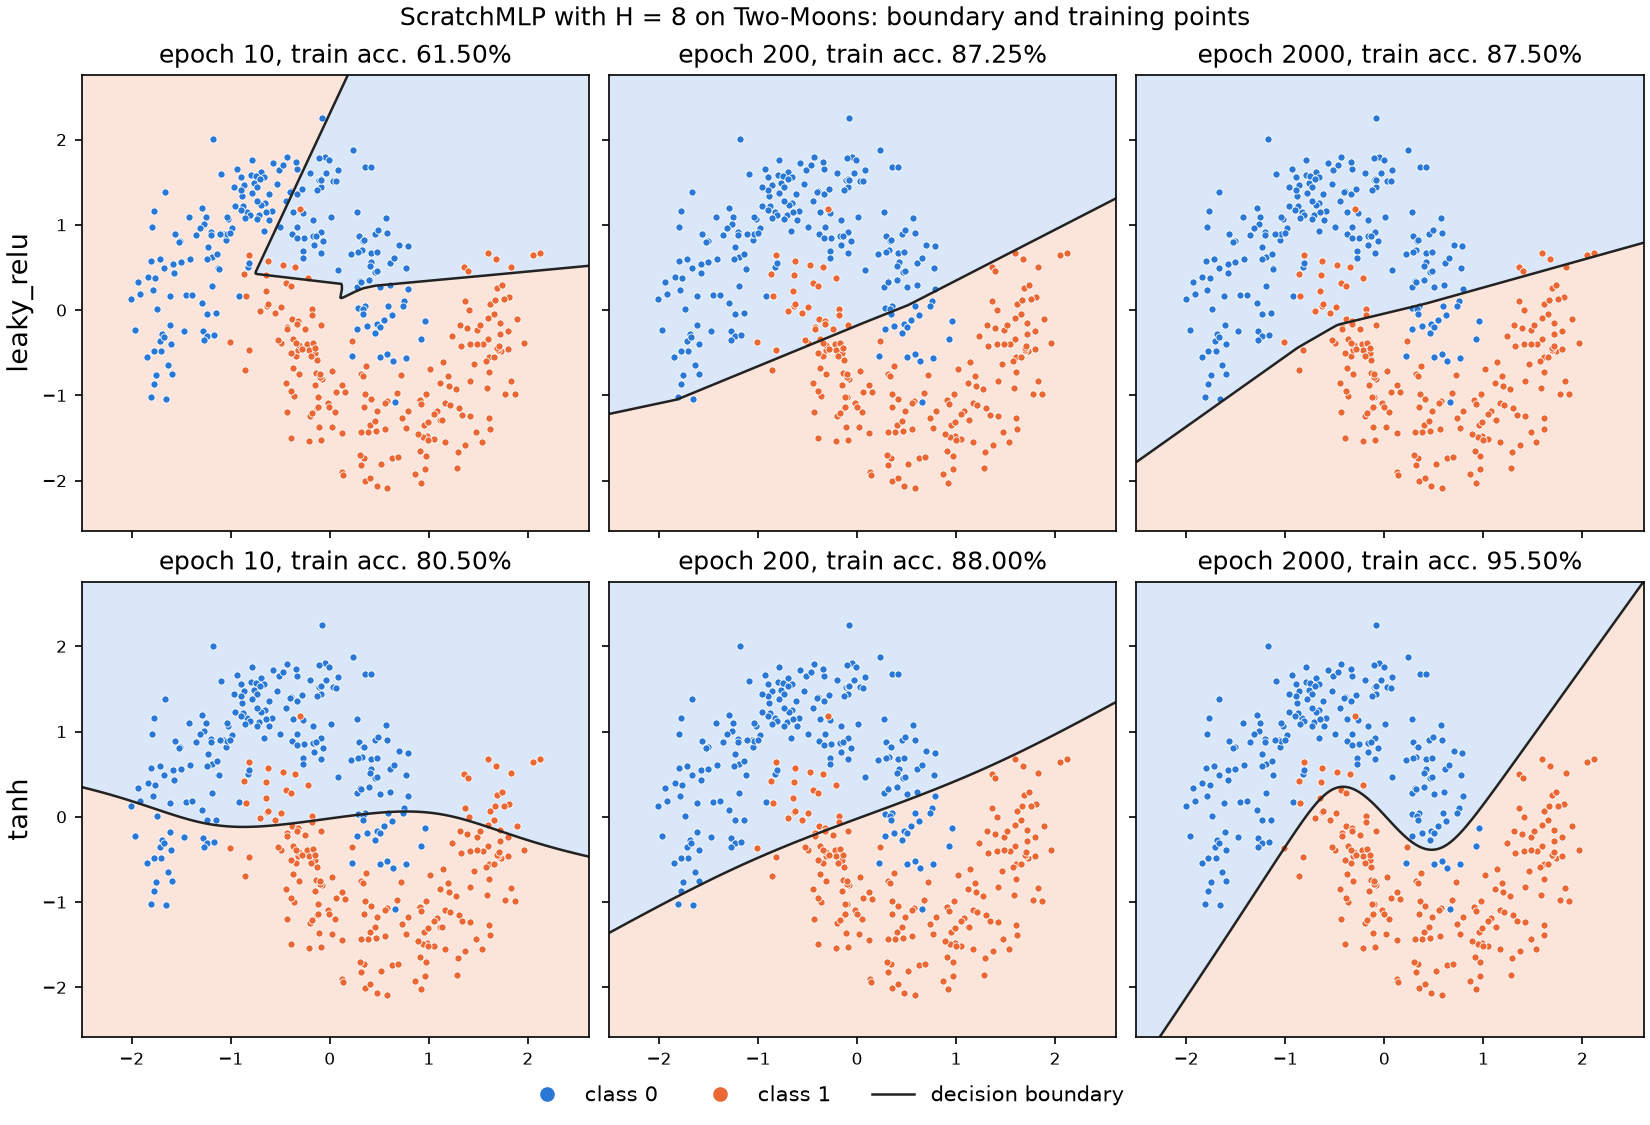
\includegraphics[width=0.72\linewidth]{../part1_boundaries.png}
  \caption{\texttt{part1\_boundaries.png}: \texttt{ScratchMLP} with $H = 8$ on Two-Moons after 10,
    200 and 2000 epochs. Top row leaky ReLU, bottom row tanh.}
\end{figure}

\begin{figure}[p]
  \centering
  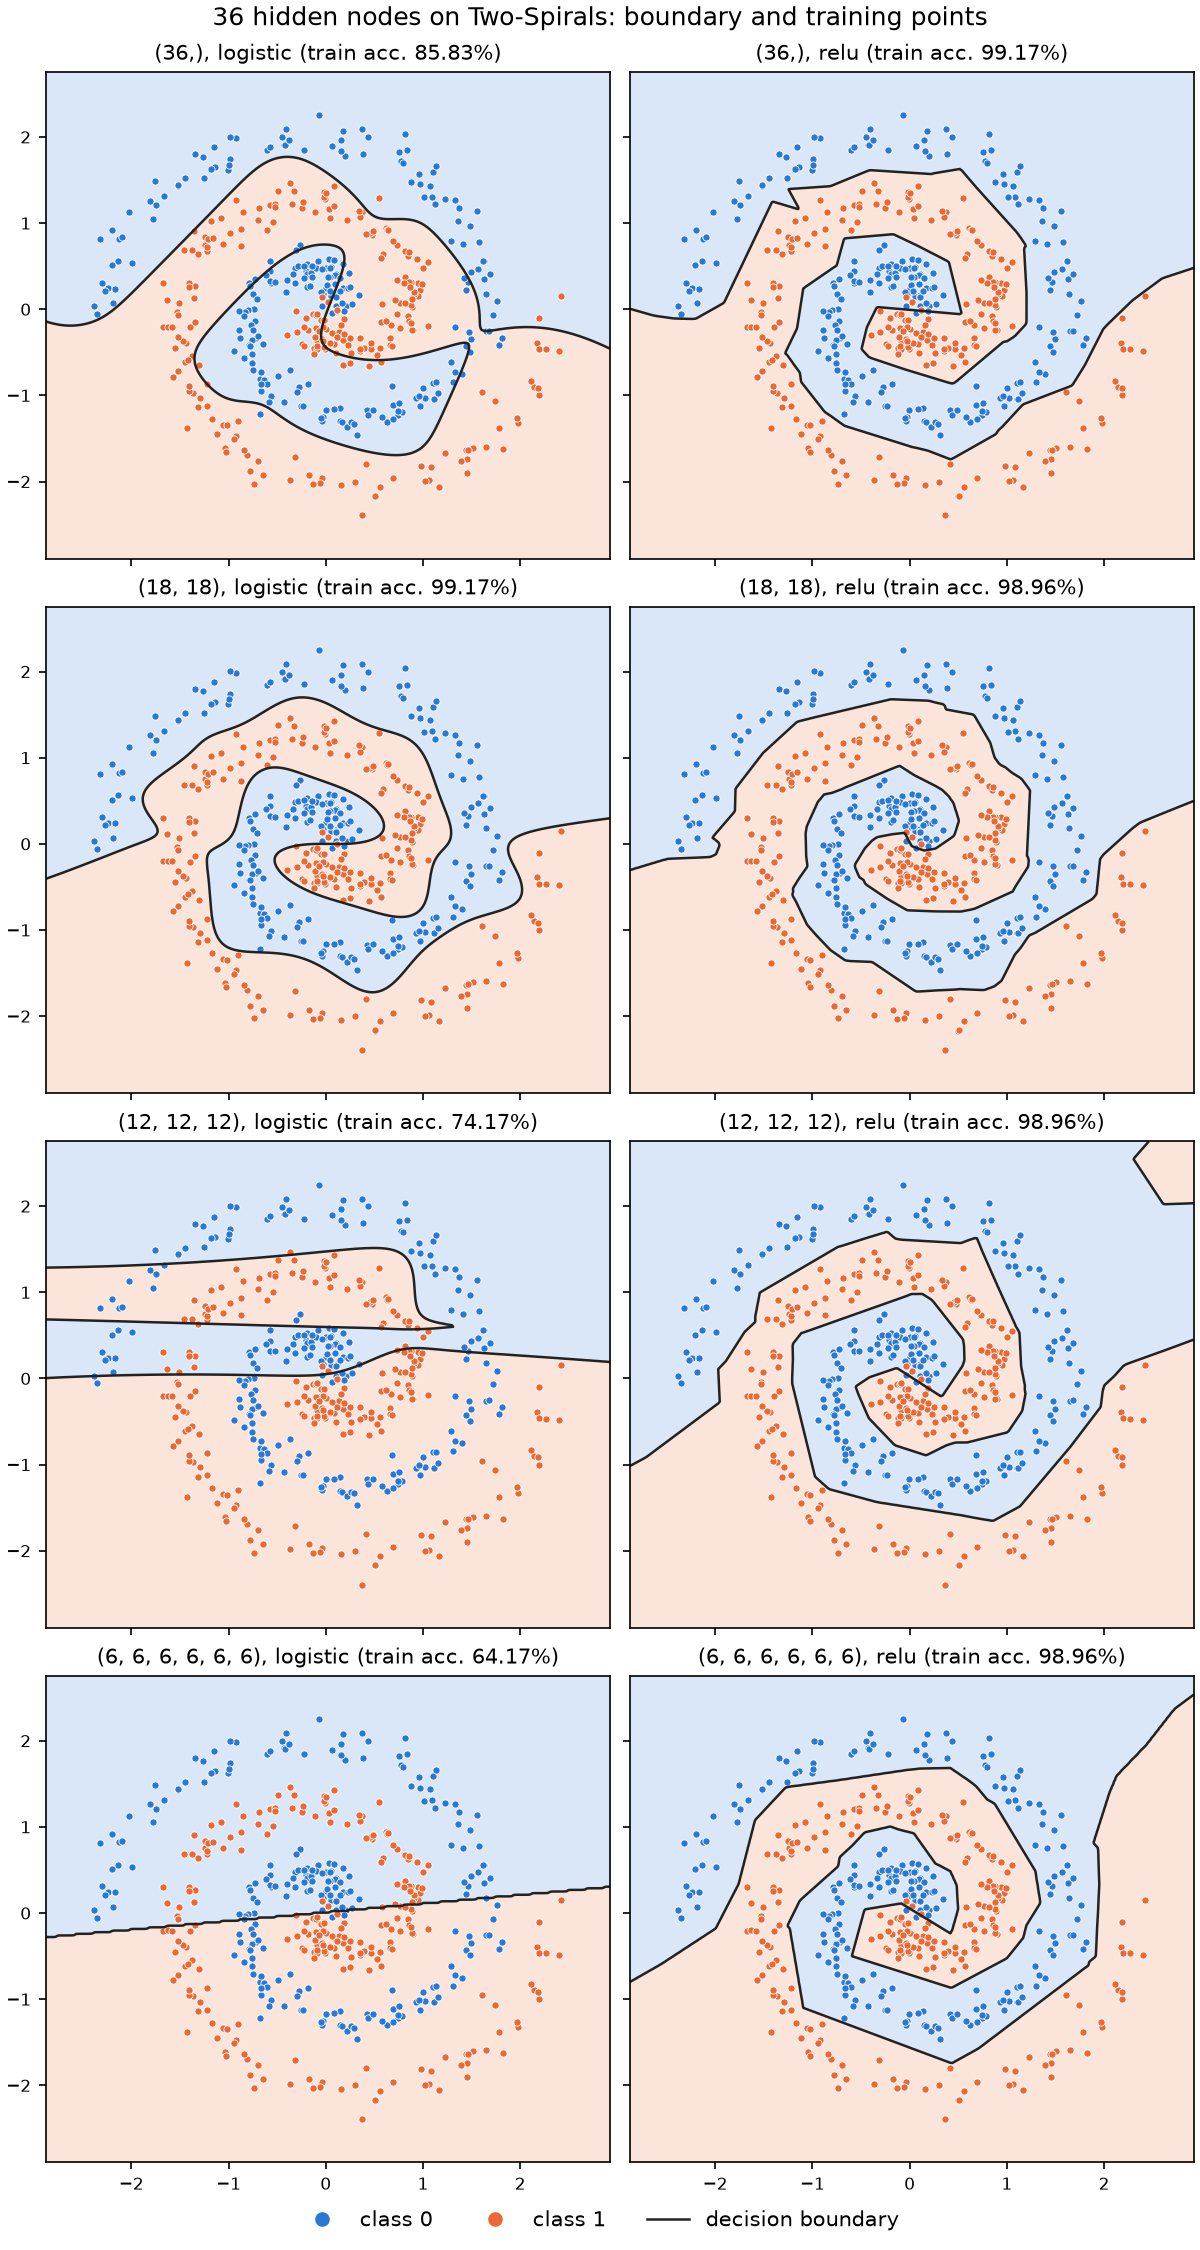
\includegraphics[height=0.9\textheight]{../part2_depth_vs_width.png}
  \caption{\texttt{part2\_depth\_vs\_width.png}: the eight models of Table~3. Rows are the
    architectures, columns the activations.}
\end{figure}

\begin{figure}[p]
  \centering
  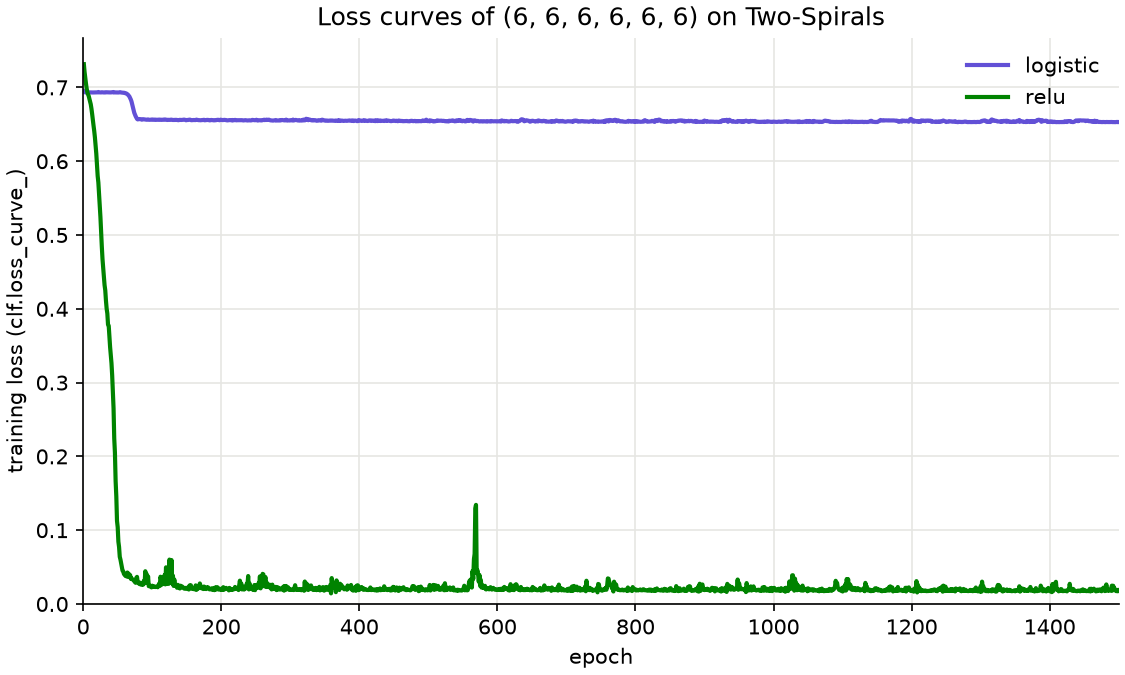
\includegraphics[width=0.7\linewidth]{../part2_loss_curves.png}
  \caption{\texttt{part2\_loss\_curves.png}: \texttt{clf.loss\_curve\_} of the deepest architecture,
    \texttt{(6, 6, 6, 6, 6, 6)}, for the two activations.}

  \vspace{1cm}
  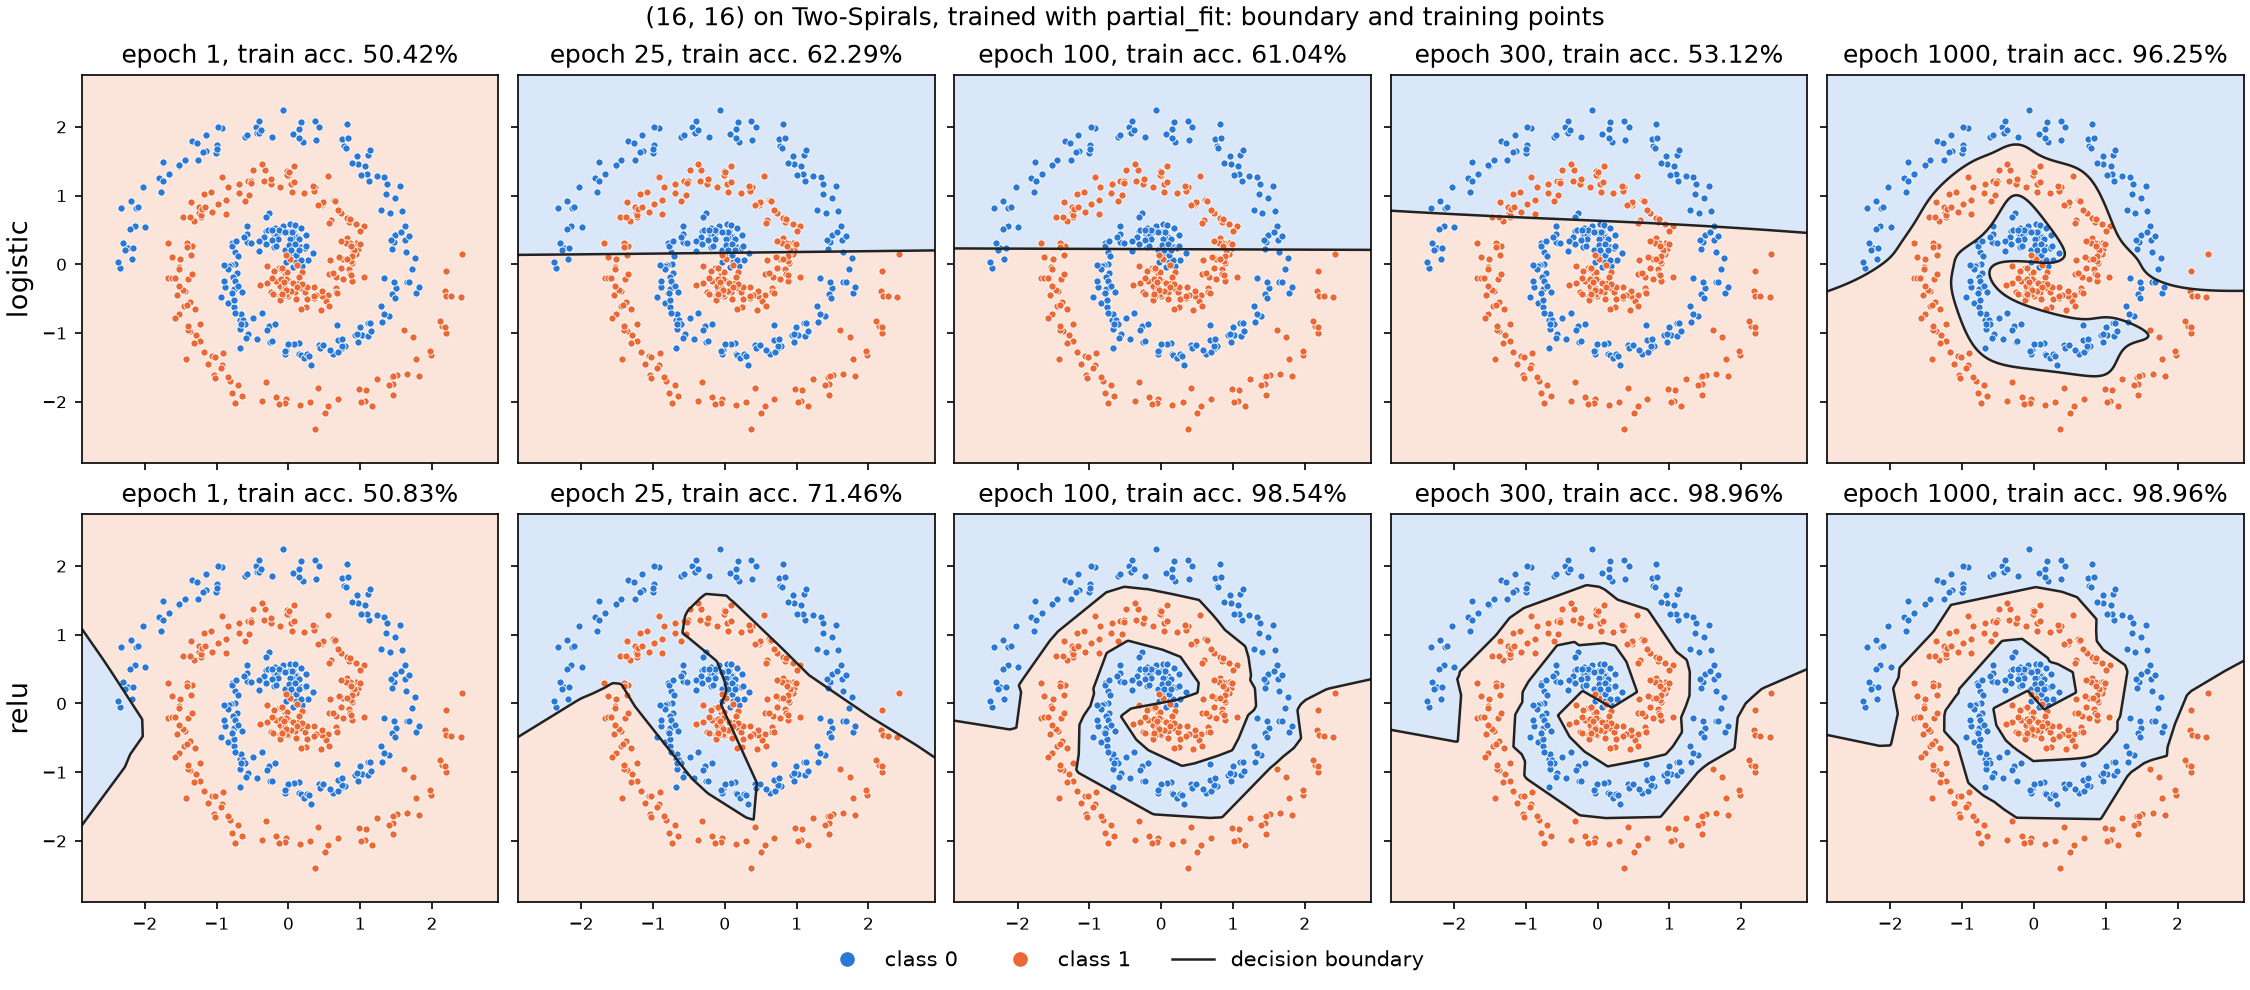
\includegraphics[width=\linewidth]{../part2_boundary_evolution.png}
  \caption{\texttt{part2\_boundary\_evolution.png}: \texttt{(16, 16)} trained with
    \texttt{partial\_fit}, after 1, 25, 100, 300 and 1000 epochs. Top row \texttt{logistic},
    bottom row \texttt{relu}.}
\end{figure}

\end{document}
